\documentclass[12pt]{article}
\usepackage{blindtext}
\usepackage[utf8]{inputenc}
\usepackage{amsmath}
\usepackage{graphicx}
\graphicspath{ {imgs/} }

\title{Tietokantasovellus-harjoitustyön dokumentaatio}


\date{\today}
\begin{document}
  \maketitle
  \newpage
  \tableofcontents
  \newpage

  \section{Johdanto}
    Tässä tietokantasovellus-harjoitustyössä tarkoituksenani on tehdä Wikipedian tyylinen järjestelmä, jossa käyttäjät voivat muokata artikkeleita eri aiheista. Jokaisesta artikkelista voi olla versio eri kielillä ja jokaiseen artikkeliin kuuluu keskustelusivu. Artikkelit muodostavat lisäksi verkon: Jokaisella artikkelilla voi olla joukko "yläartikkeleita", joiden aihepiiriin artikkeli kuuluu, ja "ala-artikkeleita", jotka kuuluvat artikkelin aihepiiriin.

    Työ toteutetaan Helsingin yliopiston users-palvelimella. Kielinä käytetään PHP:ta ja MySQL:iä. Järjestelmää käytetään selaimella, jonka riittää tukea HTML:ää. Järjestelmä toimii yhdellä tietokannalla.
  \newpage

  \section{Käyttötapaukset}
    \subsection{Käyttäjäryhmät}
      \textbf{Jokamies} on kuka tahansa, joka käyttää järjestelmää. Jokamies voi lukea artikkeleita ja keskusteluja, mutta ei muokata artikkeleita eikä osallistua keskusteluun. Jokamies voi rekisteröityä käyttäjäksi ja tietysti kirjautua sisään, jos on rekisteröitynyt. Kaikki käyttäjäryhmät ovat myös jokamiehiä.\\ \\
      \textbf{Käyttäjä} on kuka tahansa kirjautunut käyttäjä. Käyttäjällä on artikkeleihin muokkausoikeus ja mahdollisuus osallistua artikkelien keskusteluihin. Nämä oikeudet voidaan tosin myös poistaa käyttäjältä. \\ \\
      \textbf{Moderaattori} on käyttäjä, jolla on lisäksi oikeus poistaa ja muokata muiden käyttäjien viestejä ja vaihtaa artikkelista näytettävää versiota versiopuusta. \\ \\
      \textbf{Ylläpitäjä} on käyttäjä, jolla on moderointioikeuksien lisäksi oikeus muuttaa muiden käyttäjien oikeuksia, muokata kielitietokantaa.
    \subsection{Käyttötapaukset}
      \textbf{Jokamiehen käyttötapaukset:} \\
        -Artikkeleiden lukeminen \\
        -Artikkeleiden etsiminen hakutoiminnolla \\
        -Rekisteröityminen \\
        -Kirjautuminen \\ \\
      \textbf{Käyttäjän käyttötapaukset:} \\
        Jokamiehen käyttötapausten lisäksi:\\
        -Artikkelin muokkaaminen: Artikkelista on mahdollista muokata erikielisiä versioita. Muokattaessa artikkelin yläluokka-artikkeleita on mahdollista lisätä ja poistaa. (Alaluokat määräytyvät sen perusteella, mistä artikkelista kyseinen artikkeli on lisätty yläluokaksi) \\
        -Uuden artikkelin lisääminen \\
        -Viestin kirjoittaminen artikkelin keskusteluun. \\
        -Oman viestin muokkaaminen \\
        -Oman viestin poistaminen \\ \\
      \textbf{Moderaattorin käyttötapaukset:}\\
        Käyttäjän käyttötapausten lisäksi:\\
        -Artikkelin version vaihtaminen (versioksi on mahdollista vaihtaa myös "nollaversio", mikä vastaa artikkelin poistamista) \\
        -Keskusteluissa muiden viestien muokkaaminen \\
        -Keskusteluissa muiden viestien poistaminen \\ \\
      \textbf{Ylläpitäjän käyttötapaukset:}\\
        Moderaattorin käyttötapausten lisäksi:\\
        -Muiden käyttäjien käyttöoikeuksien muuttaminen \\
        -Kielitietokannan muokkaaminen \\

  \newpage
  \section{Järjestelmän tietosisältö}
        \textbf{Käsitekaavio:} \\
        \makebox[\textwidth]{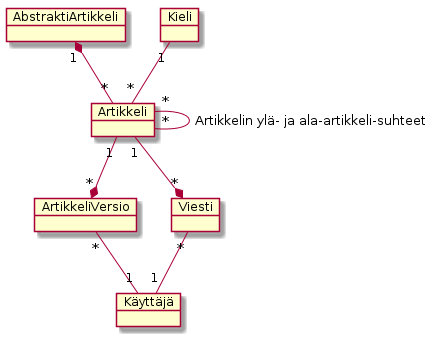
\includegraphics[width={\textwidth}]{tietos.png}}

        \textbf{Tietokohde:AbstraktiArtikkeli} \\
        AbstraktiArtikkeli on jokin tietty aihe (käytännössä vain id), josta voi olla erikielisiä artikkeleita. Jokainen artikkeli on linkitetty johonkin AbstraktiArtikkeliin. Samaan AbstraktiArtikkeliin linkitetyt erikieliset artikkelit tulkitaan olevan samasta aiheesta tehtyjä erikielisiä versioita. Jos samaan AbstraktiArtikkeliin on linkitetty kaksi samankielistä artikkelia, näiden tulkitaan olevan päällekkäinen versio samasta aiheesta. \\ \\
        \textbf{Tietokohde:Artikkeli}\\
        \begin{tabular}{|p{8em}|p{8em}|p{13em}|} \hline
            \textbf{Attribuutti} & \textbf{Arvojoukko} & \textbf{Kuvailu} \\ \hline
                    abstraktiArtikkeli
                &   AbstraktiArtikkeli
                &   Artikkelin "aihe".
            \\ \hline
                    kieli
                &   Kieli
                &   Kieli, millä artikkeli on kirjoitettu
            \\ \hline
                    nimi
                &   merkkijono
                &   Artikkelin nimi
            \\ \hline
        \end{tabular} \\ \\ \\

        \textbf{Tietokohde:ArtikkeliVersio} \\
        \begin{tabular}{|p{8em}|p{8em}|p{13em}|} \hline
            \textbf{Attribuutti} & \textbf{Arvojoukko} & \textbf{Kuvailu} \\ \hline
                    artikkeli
                &   Artikkeli
                &   Tunniste, minkä artikkelin versio tämä on
            \\ \hline
                    edellinenVersio
                &   ArtikkeliVersio
                &   Tunniste, mikä on edellinen versio tästä artikkelista
            \\ \hline
                    luoja
                &   Käyttjää
                &   Käyttäjä, joka on luonut tämän version artikkelista
            \\ \hline
                    Teksti
                &   merkkijono
                &   Artikkelin teksti
            \\ \hline
        \end{tabular} \\ \\ \\

        \textbf{Tietokohde:Kieli} \\
        \begin{tabular}{|p{8em}|p{8em}|p{13em}|} \hline
            \textbf{Attribuutti} & \textbf{Arvojoukko} & \textbf{Kuvailu} \\ \hline
                    nimi
                &   merkkijono
                &   Kielen nimi
            \\ \hline
        \end{tabular} \\ \\ \\

        \textbf{Tietokohde:Kieli} \\
        \begin{tabular}{|p{8em}|p{8em}|p{13em}|} \hline
            \textbf{Attribuutti} & \textbf{Arvojoukko} & \textbf{Kuvailu} \\ \hline
                    nimi
                &   merkkijono
                &   Kielen nimi
            \\ \hline
        \end{tabular} \\ \\ \\

        \textbf{Tietokohde:Viesti} \\
        \begin{tabular}{|p{8em}|p{8em}|p{13em}|} \hline
            \textbf{Attribuutti} & \textbf{Arvojoukko} & \textbf{Kuvailu} \\ \hline
                    artikkeli
                &   Artikkeli
                &   Artikkeli, jonka keskusteluun viesti on jätetty
            \\ \hline
                    kirjoittaja
                &   Käyttäjä
                &   Viestin kirjoittanut käyttäjä
            \\ \hline
                    viesti
                &   merkkijono
                &   Viestin sisältö
            \\ \hline
        \end{tabular} \\ \\ \\


        \textbf{Tietokohde:Käyttäjä} \\
        \begin{tabular}{|p{8em}|p{8em}|p{13em}|} \hline
            \textbf{Attribuutti} & \textbf{Arvojoukko} & \textbf{Kuvailu} \\ \hline
                    käyttäjänimi
                &   merkkijono
                &   Uniikki käyttäjänimi
            \\ \hline
                    sähköposti
                &   merkkijono
                &   sähköpostiosoite
            \\ \hline
                    salasana
                &   merkkijono
                &   salasanan tiiviste
            \\ \hline
        \end{tabular}
  \newpage

  \section{Relaatiotietokantakaavio}
        \makebox[\textwidth]{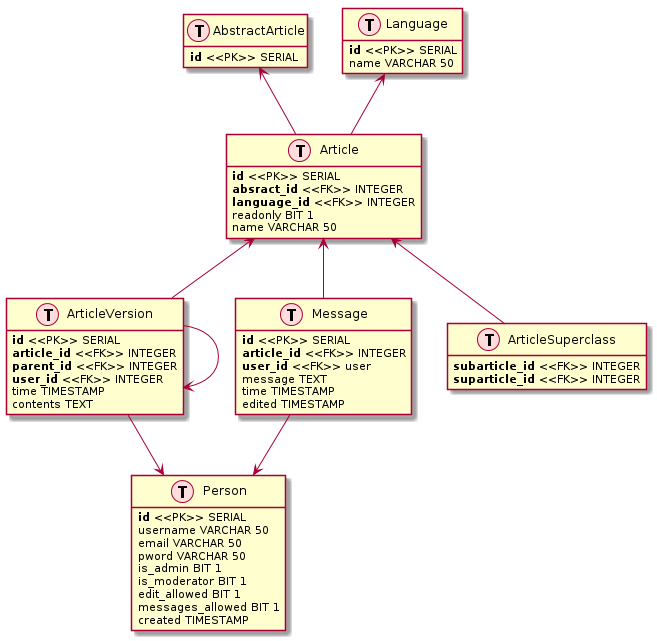
\includegraphics[width={\textwidth}]{relt.png}} \\
        Tietosisällön käsitekaavioon verrattuna relaatiotietokantakaavioon on lisätty article\_superclass, jota käsitekaaviossa mallintaa yhteys artikkelista itseensä.
        

\end{document}
\grid
\grid
\grid
